\chapter{Return estimation}

This chapter summarizes the first step in strategic asset allocation - estimation of future returns' probability density function. We will cover everything from data import to the drawing/simulation of future returns from an estimated distribution.

\section{The data}

The data available at our disposal consist of daily returns dating back almost two decades for eight representative asset classes. In the spirit of our modular approach, the investor is able to input their own return observations and preferred asset classes into our framework. Throughout this chapter, however, we will assume a given set of eight asset classes and explain our future return estimation mechanics on this particular asset class set.

The assets used in our analysis contain indices following the prices of gold, US Treasury bonds, a specific ASW portfolio, world equity, Chinese government bonds, US Inflation-linked government bonds, Mortgage-backed securities and emerging markets. These are all summarized in Table \ref{tab:return_estimation:asset_classes} and form our basic 8 available asset classes.
\begin{table}[h]
	\centering
	\begin{tabularx}{0.9\linewidth}{rX}
		Asset class & Relevant index\\
		\toprule
		\textbf{Gold} & Gold XAU/EUR Rate FX Unhdg.
		 \\
		\textbf{US} & 1-5 Year US Govt (ICE) FX Unhdg.
		 \\
		\textbf{ASW} & 1-5 Year Global Non-Sov (ICE) IR hdg. IRS
		 \\
		\textbf{Stocks} & World Equity (MSCI) FX Unhdg.
		\\
		\textbf{China} & 1-3 Year China Govt (ICE) FX Unhdg.
		\\
		\textbf{InflBonds} & US Inflation-Linked Govt (ICE) FX Hdg.
		\\
		\textbf{MBS} & US MBS (ICE) FX Hdg.
		 \\
		\textbf{EM} & EM global IG Govt (JPM) FX Hdg.
		 \\
		
		\bottomrule
	\end{tabularx}
	\caption{Asset classes.}
	\label{tab:return_estimation:asset_classes}
\end{table}

\section{The return simulation process}

Following consecutive steps are part of the return estimation process:

\begin{table}[h]
	\centering
	\begin{tabularx}{0.9\linewidth}{lXX}
		Parameter & Description & Default value\\
		\toprule
		\textbf{N\_simulation} & Number of returns that are being simulated. From these, the final returns are drawn uniformly randomly, depending on sample size. Therefore must be greater than $\max\left[\text{sample\_sizes}\right]$. & 1 000 000
		\\
		\textbf{sample\_sizes} & Sample sizes for which future returns are simulated. & (100, 500, 1000, 2000, 5000, 10000, 50000, 100000) 
		\\
		\textbf{maturities} & Maturities for which future returns are simulated.& (1,3,6,12,60) 
		\\
		\textbf{frequency} & Frequency to which daily historical returns are being transformed first. & monthly
		\\
		\textbf{selected\_copula\_types} & Selection of available copula families that are allowed to be used within the model selection procedure. & all copulas available in the VineCopula package for R
		\\
		\bottomrule& 
	\end{tabularx}
	\caption{User parameters used in return estimation and simulation.}
	\label{tab:return_estimation:user_parameters}
\end{table} 
\begin{enumerate}
	\item User parameters specified. These include the sample size of simulated future return distribution, maturity of said returns, frequency of historical returns used in such estimation etc. For a full list of relevant user parameters, see Table \ref{tab:return_estimation:user_parameters}.
	\item Imported daily data.
	\item Created a new dataset with observation frequency chosen by the user - daily, weekly, monthly or yearly. Data saved in a relevant folder.
	\item Fit each asset class with both Gaussian as well as Pearson type VII distribution.
	\item Transform each asset class into a $[0,1]$ uniformly distributed variable using the distributional assumption of a Pearson type VII distribution.
	\item Fit the copula to the uniformly distributed marginal data, drawing from the allowed copula families selected by the user.
	\item Use the fitted model to generate $N\_simulation$ observations of simulated returns / draw them from the estimated distibution. Also draw the same number of returns from multidimensional Gaussian distribution.
	\item Plot pairwise correlations of the simulated Pearson + Copula vs. Gaussian returns vs. historical data to allow for a visual comparison.
	\item Compute the Cramer and Kolmogorov-Smirnov tests on distributional equality to evaluate the similarity of simulated return distribution to the original distribution.
	\item Use the simulated returns to create datasets with different maturities and sample sizes - daily, weekly, monthly and yearly. Save them in a pre-specified directory structure together with the relevant estimated copula structure.
\end{enumerate}

This process can also be schematically viewed as an algorithm in Algorithm \ref{alg:return_estimation}. Several steps in this procedure however warrant further clarification and details, which we shall focus on in the following paragraphs.

\begin{algorithm}[!htb]
	\KwData{historical returns}
	\KwIn{N\_simulation, sample sizes, maturities, frequency, copula\_types}
	\KwResult{simulated returns}
	import historical return data\;
	\eIf{frequency=="daily"}{
		no aggregation;
	}{
		\eIf{frequency=="weekly"}{
			aggregate to weekly returns\;
		}{
			\If{frequency=="monthly"}{
				aggregate to monthly returns\;
			}
		}
	}
	set custom asset names\;
	create directory structure\;
	save aggregated	data\;
	\ForEach{asset class}{
		estimate the Pearson and Gaussian distribution parameters\;
		generate simulated returns from Pearson and Gaussian distribution\;
		plot marginal historical return distribution with Pearson and Gaussian fit\;
		transform asset class to a $[0,1]$ uniform distribution\;
	}
	fit a multivariate Gaussian distribution to the data;\
	fit the copula to the uniform data, drawing from allowed copula types\;
	plot historical vs. simulated returns in a pairwise correlation plot\;
	run a Cramer test on equality of distributions with the historical data for both models (Gaussian and copula)\;
	\ForEach{asset class}{
		run a Kolmogorov-Smirnov test of distributional equality with the historical data for both models\;
	}
	save results of Cramer and K-S tests\;
	\For{sample sizes}{
		\For{maturities}{
			store the simulated returns in the relevant path;\
			acording to the frequency, compute the p.a. returns and store them in the appropriate path\;			
		}
	}
	store the copula structure\;
	\caption{Return estimation and simulation.}
	\label{alg:return_estimation}
\end{algorithm}

The data on historical returns is stored as a \textit{historical\_daily\_returns.csv} file with columns corresponding to the different asset classes and rows corresponding to daily returns. Furthermore, we also use an input file called \textit{portfolio\_constraints.xlsx} which besides relevant default investor constraints also contains short versions of the respective asset class names.

In the first step, the returns are loaded into R, formatted as numeric values and transformed to a desired frequency chosen by the user. The transformation from daily observations to e.g. weekly observations is done by:
\begin{enumerate}
	\item adding 1 to each observation,
	\item multiplying the observations corresponding to a particular week,
	\item subtracting 1 from the result.
\end{enumerate}
The new dataframe is now taken as a baseline. We assign custom asset class names to all variables (taken from \textit{portfolio\_constraints.xlsx}) and save this dataset in an appropriate data folder (for directory structure of the project, refer to the technical summary at the end of this report).

In the second step, we estimate both the Pearson and Gaussian marginal distributions that are the best fits for our data. A one-dimensional Gaussian distribution has the following density function:

\begin{equation}
f(x)={\frac {1}{\sigma {\sqrt {2\pi }}}}e^{-{\frac {1}{2}}\left({\frac {x-\mu }{\sigma }}\right)^{2}}
\end{equation}

where $\mu$ is the expected value and $\sigma$ is the variance of the distribution. We compute these quantities from the sample for each asset class and hence obtain the desired Gaussian distribution parameters.

A Pearson type VII distribution density is slightly more complicated, with three parameters instead of two:


\begin{equation}
f(x\mid \lambda, \alpha, m)={\frac {1}{\alpha \operatorname {\mathrm {B} } \left(m-{\frac {1}{2}},{\frac {1}{2}}\right)}}\left[1+\left({\frac {x-\lambda }{\alpha }}\right)^{2}\right]^{-m}
\end{equation}

The benefits associated with this distribution mostly lie in its scalability with respect to its fourth moment - kurtosis. This freedom allows us to better approximate the historical returns not only in their mean and variance, but also in terms of their tails. This property is especially crucial if we are dealing with investor that places high importance on tail-relevant risk measures such as Value-at-Risk or expected shortfall. In light of such preferences, having a reliable way of predicting tail events is of utmost importance.

An alternative parameterization of the Pearson type VII distribution can be achieved by substituting $\alpha := \sigma\sqrt{2m-3}$. In such case, letting $m$ approach the infinity provides us with a well-known Gaussian distribution as the kurtosis approaches the value of 3. Assuming $m>5/2$ guarantees the existence of the distributions' first four moments. Another substitution of $\lambda=\mu, \alpha=\sqrt{\nu\sigma^2}, m=\frac{\nu+1}{2}$ then gives us the non-standardized Student's t distribution
\begin{equation}
f(x\mid \mu ,\sigma ^{2},\nu )={\frac {1}{{\sqrt {\nu \sigma ^{2}}}\,\operatorname {\mathrm {B} } \left({\frac {\nu }{2}},{\frac {1}{2}}\right)}}\left(1+{\frac {1}{\nu }}{\frac {(x-\mu )^{2}}{\sigma ^{2}}}\right)^{-{\frac {\nu +1}{2}}}
\end{equation}
After some basic algebraic computations, we can show that a random variable $X$ with this particular distribution has its first four moments given by the following formulae:
\begin{eqnarray}
	\text{E}[X] &=& \mu \\ 
	\text{Var}[X] &=& \sigma^2\frac{\nu}{\nu-2} \\
	\text{Skew}[X] &=& 0 \\
	\text{Kurt}[X] &=& \frac{3\nu-6}{\nu-4}
\end{eqnarray}
With this in mind, we can estimate parameters $\mu, \sigma$ and $\nu$ from the first four moments of historical returns simply by letting these expressions be equal to sample-specific moments. With the distribution successfully parameterized, we can easily draw an arbitrary number of simulated returns from the estimated distribution.


\begin{figure}[!htb]
	\begin{subfigure}{.49\textwidth}
		\centering
		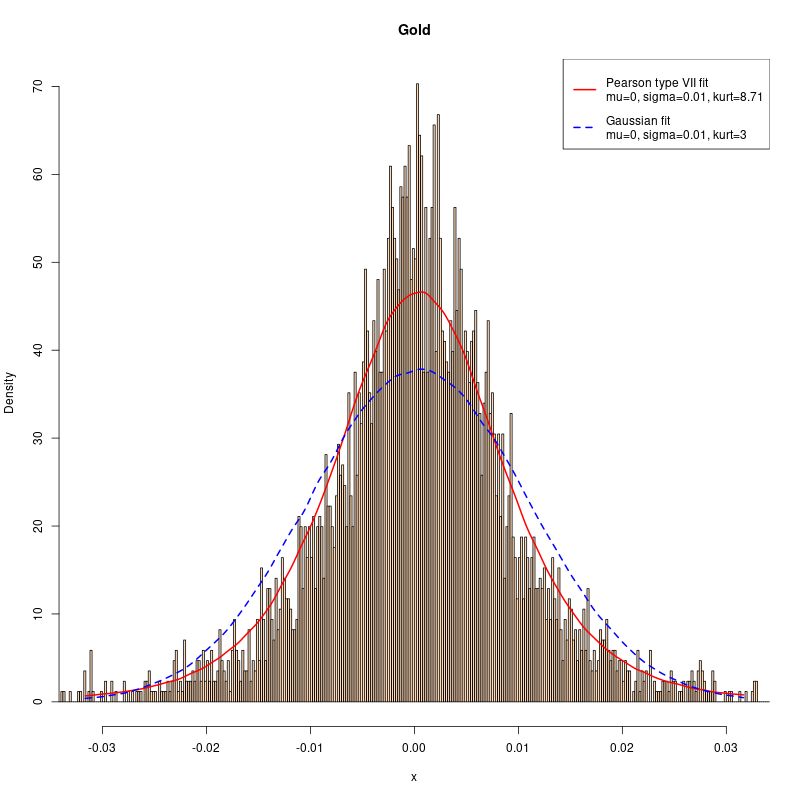
\includegraphics[width=\textwidth]{\detokenize{figures/marginal_distributions/Gold}}
		\caption{Gold}	
	\end{subfigure}
	\begin{subfigure}{.49\textwidth}
		\centering
		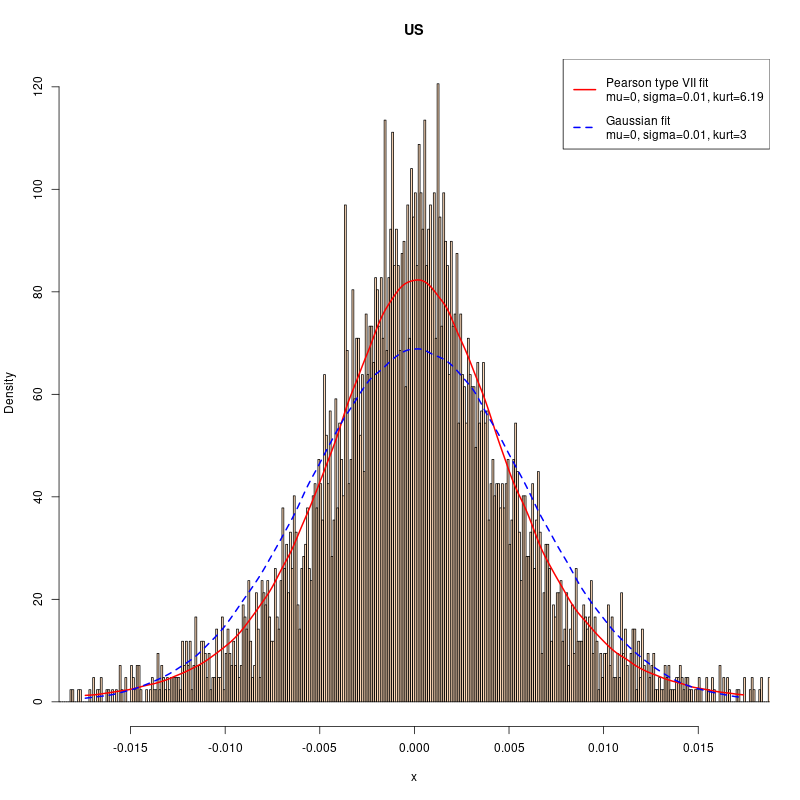
\includegraphics[width=\textwidth]{\detokenize{figures/marginal_distributions/US}}
		\caption{US Government Bonds}
	\end{subfigure}\\
	\begin{subfigure}{.49\textwidth}
		\centering
		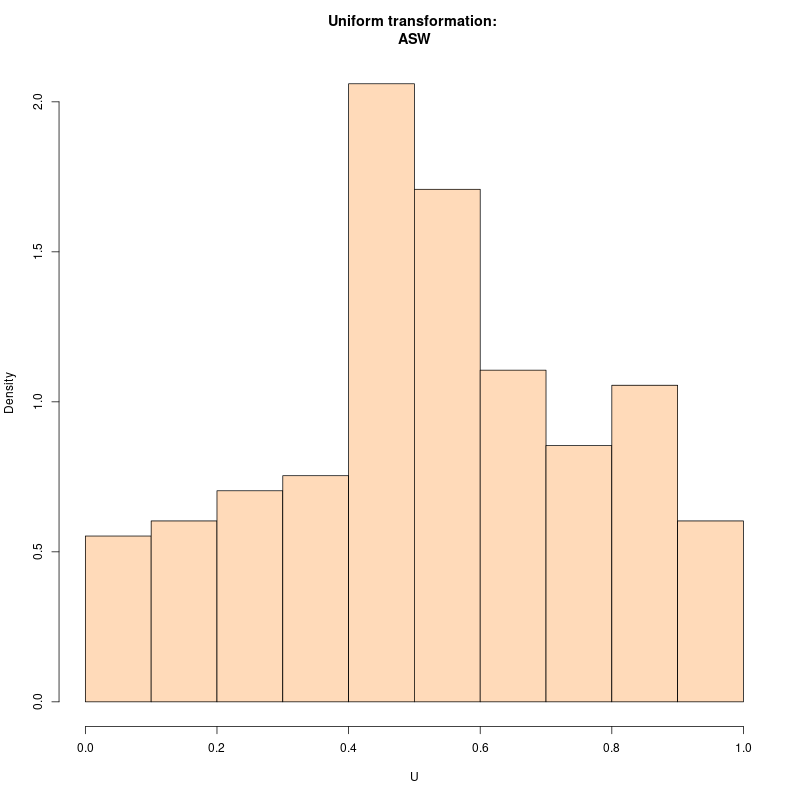
\includegraphics[width=\textwidth]{\detokenize{figures/marginal_distributions/ASW}}
		\caption{ASW portfolio}
	\end{subfigure}
	\begin{subfigure}{.49\textwidth}
		\centering
		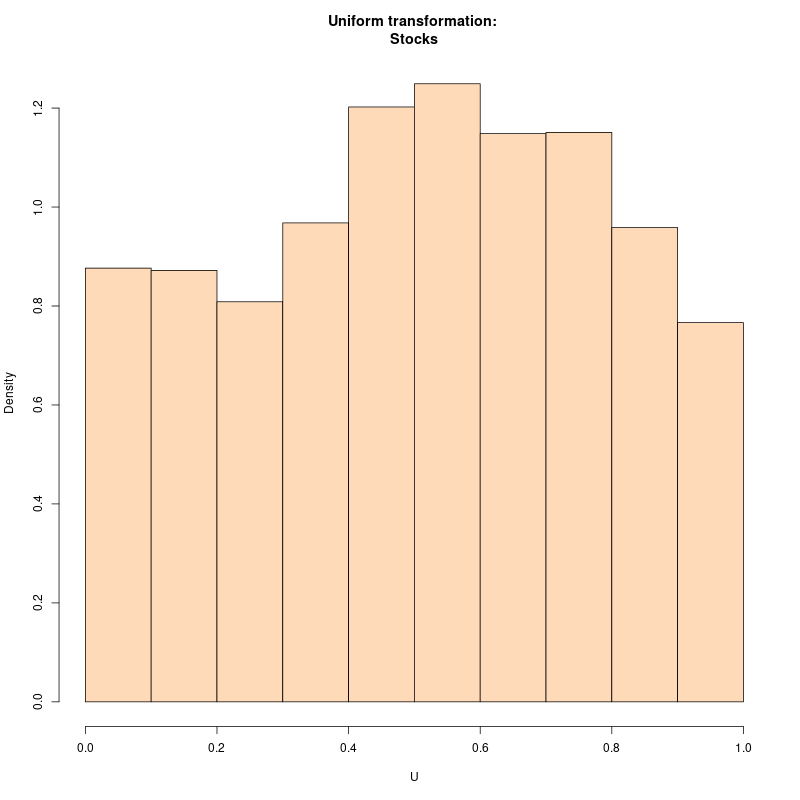
\includegraphics[width=\textwidth]{\detokenize{figures/marginal_distributions/Stocks}}
		\caption{World Equity}
	\end{subfigure}
	\caption{Historical returns, density approximated with a Gaussian and Pearson distributions. Part 1/2.}
	\label{fig:return_estimation:marginal_distributions_1}
\end{figure}
\begin{figure}[!htb]
	\begin{subfigure}{.49\textwidth}
		\centering
		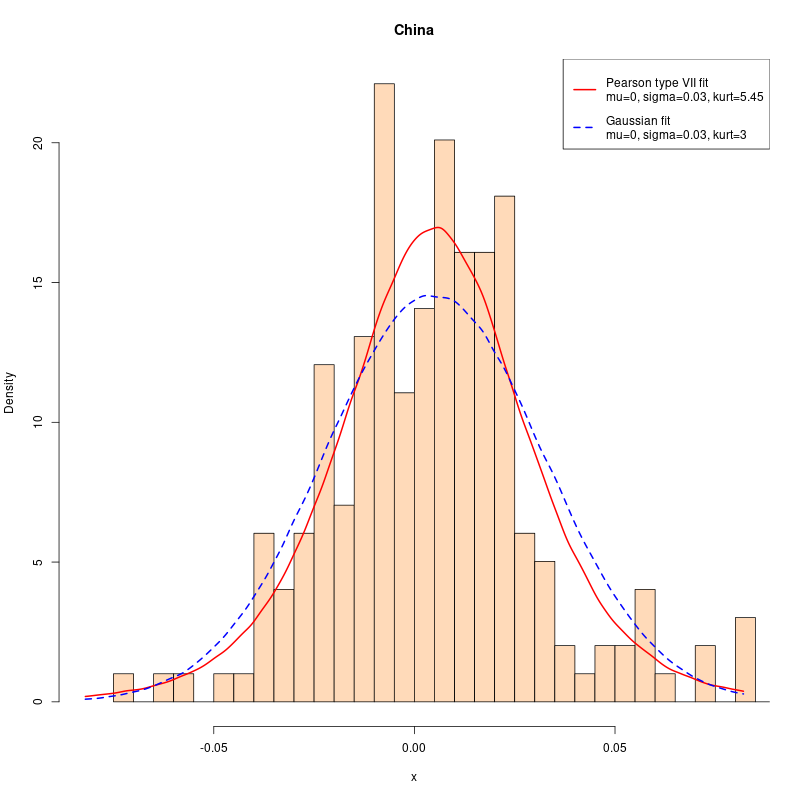
\includegraphics[width=\textwidth]{\detokenize{figures/marginal_distributions/China}}
		\caption{China Government Bonds}
	\end{subfigure}
	\begin{subfigure}{.49\textwidth}
		\centering
		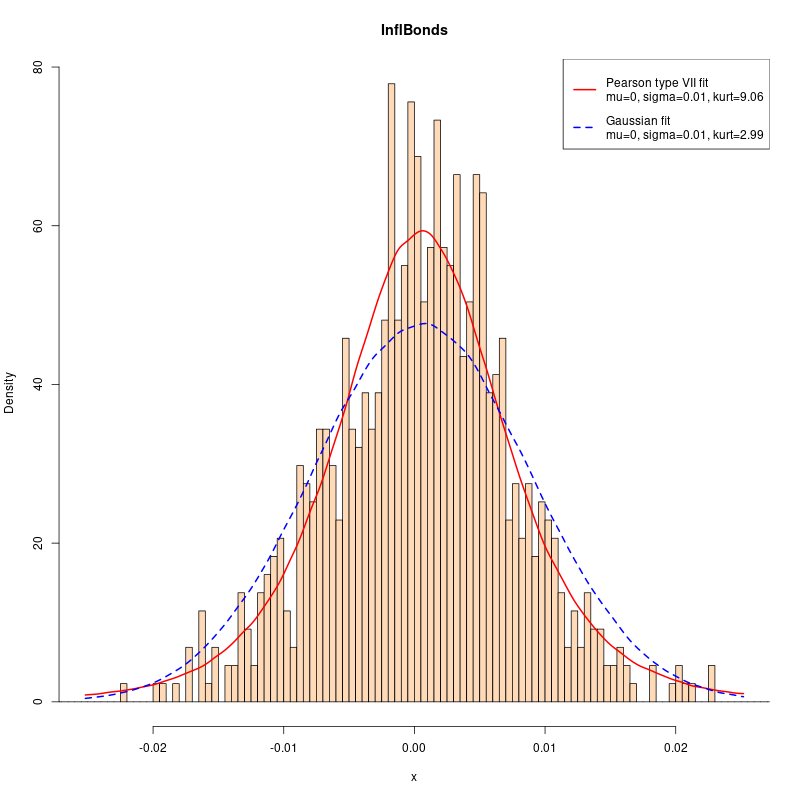
\includegraphics[width=\textwidth]{\detokenize{figures/marginal_distributions/InflBonds}}
		\caption{US Inflation-linked Government Bonds}
	\end{subfigure}\\
	\begin{subfigure}{.49\textwidth}
		\centering
		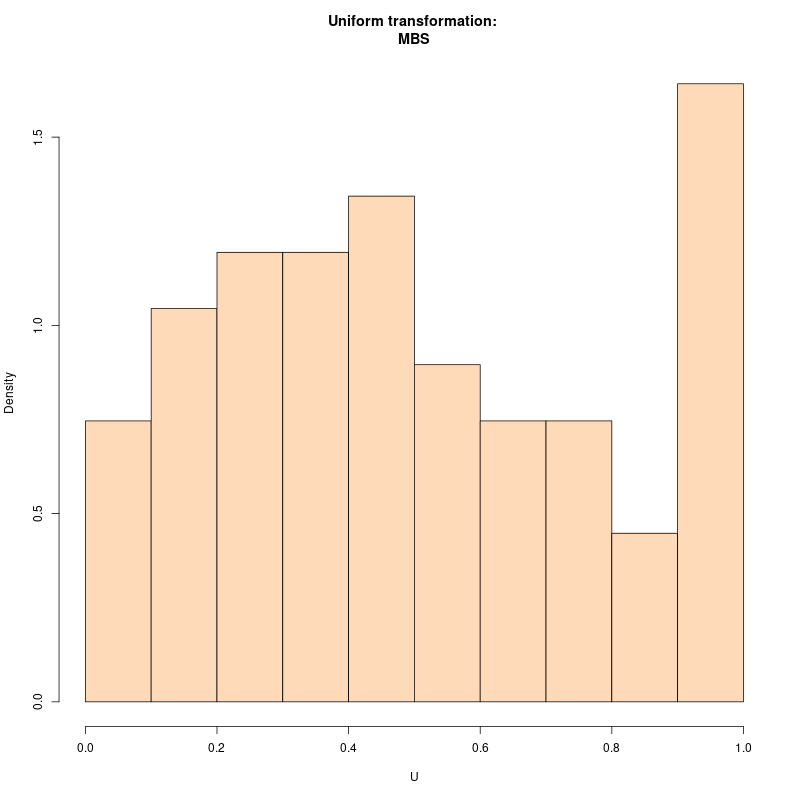
\includegraphics[width=\textwidth]{\detokenize{figures/marginal_distributions/MBS}}
		\caption{US Mortgage-backed Securities}
	\end{subfigure}
	\begin{subfigure}{.49\textwidth}
		\centering
		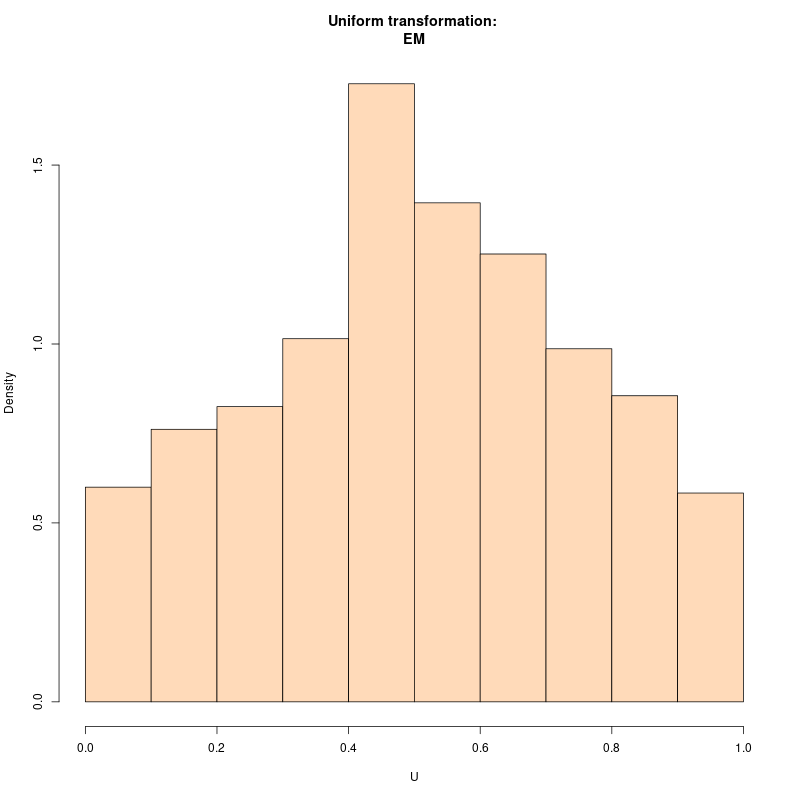
\includegraphics[width=\textwidth]{\detokenize{figures/marginal_distributions/EM}}
		\caption{Emerging markets}
	\end{subfigure}
	\caption{Historical returns, density approximated with a Gaussian and Pearson distributions. Part 2/2}
	\label{fig:return_estimation:marginal_distributions_2}
\end{figure}


Figures \ref{fig:return_estimation:marginal_distributions_1} and \ref{fig:return_estimation:marginal_distributions_2} show the relevant fit for both the Gaussian as well as the Pearson (non-standardized Student's t) distribution. The blue line corresponds to the Gaussian distribution, while the red line shows the fit of the Pearson type VII distribution.

We see that - in line with our expectations - using a distribution with variable kurtosis parameter allows for a tighter fit, especially in asset classes with fatter tails. But even though a brief visual examination is a great tool, we will also look into this goodness of fit more formally with proper statistical tests.

Before doing so, however, we shall focus on estimating the whole multidimensional distribution, not just the marginals. Again, we will do this for both the Pearson as well as the Gaussian distribution. In the former case, we shall use vine copulas for mutual pairwise dependencies, while in the latter case, we would estimate parameters of multivariate Gaussian distribution directly.

Starting with the Pearson distribution, we first transform each asset class into a $[0,1]$ uniform variable which is a necessary first step for fitting a copula model. The process is simply achieved by taking the estimated Pearson distribution function from the previous step and evaluating it at the respective historical return data points. In other words, if the random variable $X$ corresponds to our historical returns with assumed Pearson type VII cumulative distribution function $F(x)$, then the new random variable obtained by:
\begin{equation}
	U = F(X)
\end{equation}
is uniformly distributed at its domain $[0,1]$.
Transforming all asset classes this way shrinks our 8-dimensional real space into an 8-dimensional unit cube $[0,1]^8$. 

With the data transformed to a unit cube, we take advantage of the R package "Vine Copula", see \citep{2021VineCopulaPackage}. This package contains functions and routines focused on estimation and model selection of multivariate pairwise copulas also called the vine copulas. The function "\textit{RVineStructureSelect}" allows us to use its heuristical model-selection algorithm which automatically chooses and estimates the best pairwise copula model for our dataset given our choice of allowed copula families. Further details regarding the algorithm and the package in general can be found in \citep{2013Dissmann}.

Once the model is fitted, we draw N\_simulation returns from their estimated joint distribution. We follow the same approach with the multivariate Gaussian distribution, only instead of pairwise copulas, we simply use the maximum likelihood approach to estimate the distribution's vector of mean returns $\mu$ and the variance-covariance matrix $\Sigma$.

At this point, we have three sets of returns at our disposal: historical returns, Pearson type VII distributed returns with their mutual dependency given by pairwise copulas and a return set with multivariate Gaussian distribution. Pairwise dependency plot of these 3 classes of returns can be found in Figure \ref{fig:return_estimation:correlations}.

\begin{figure}[!htb]
	\centering
	\begin{subfigure}{.75\columnwidth}
		\centering
		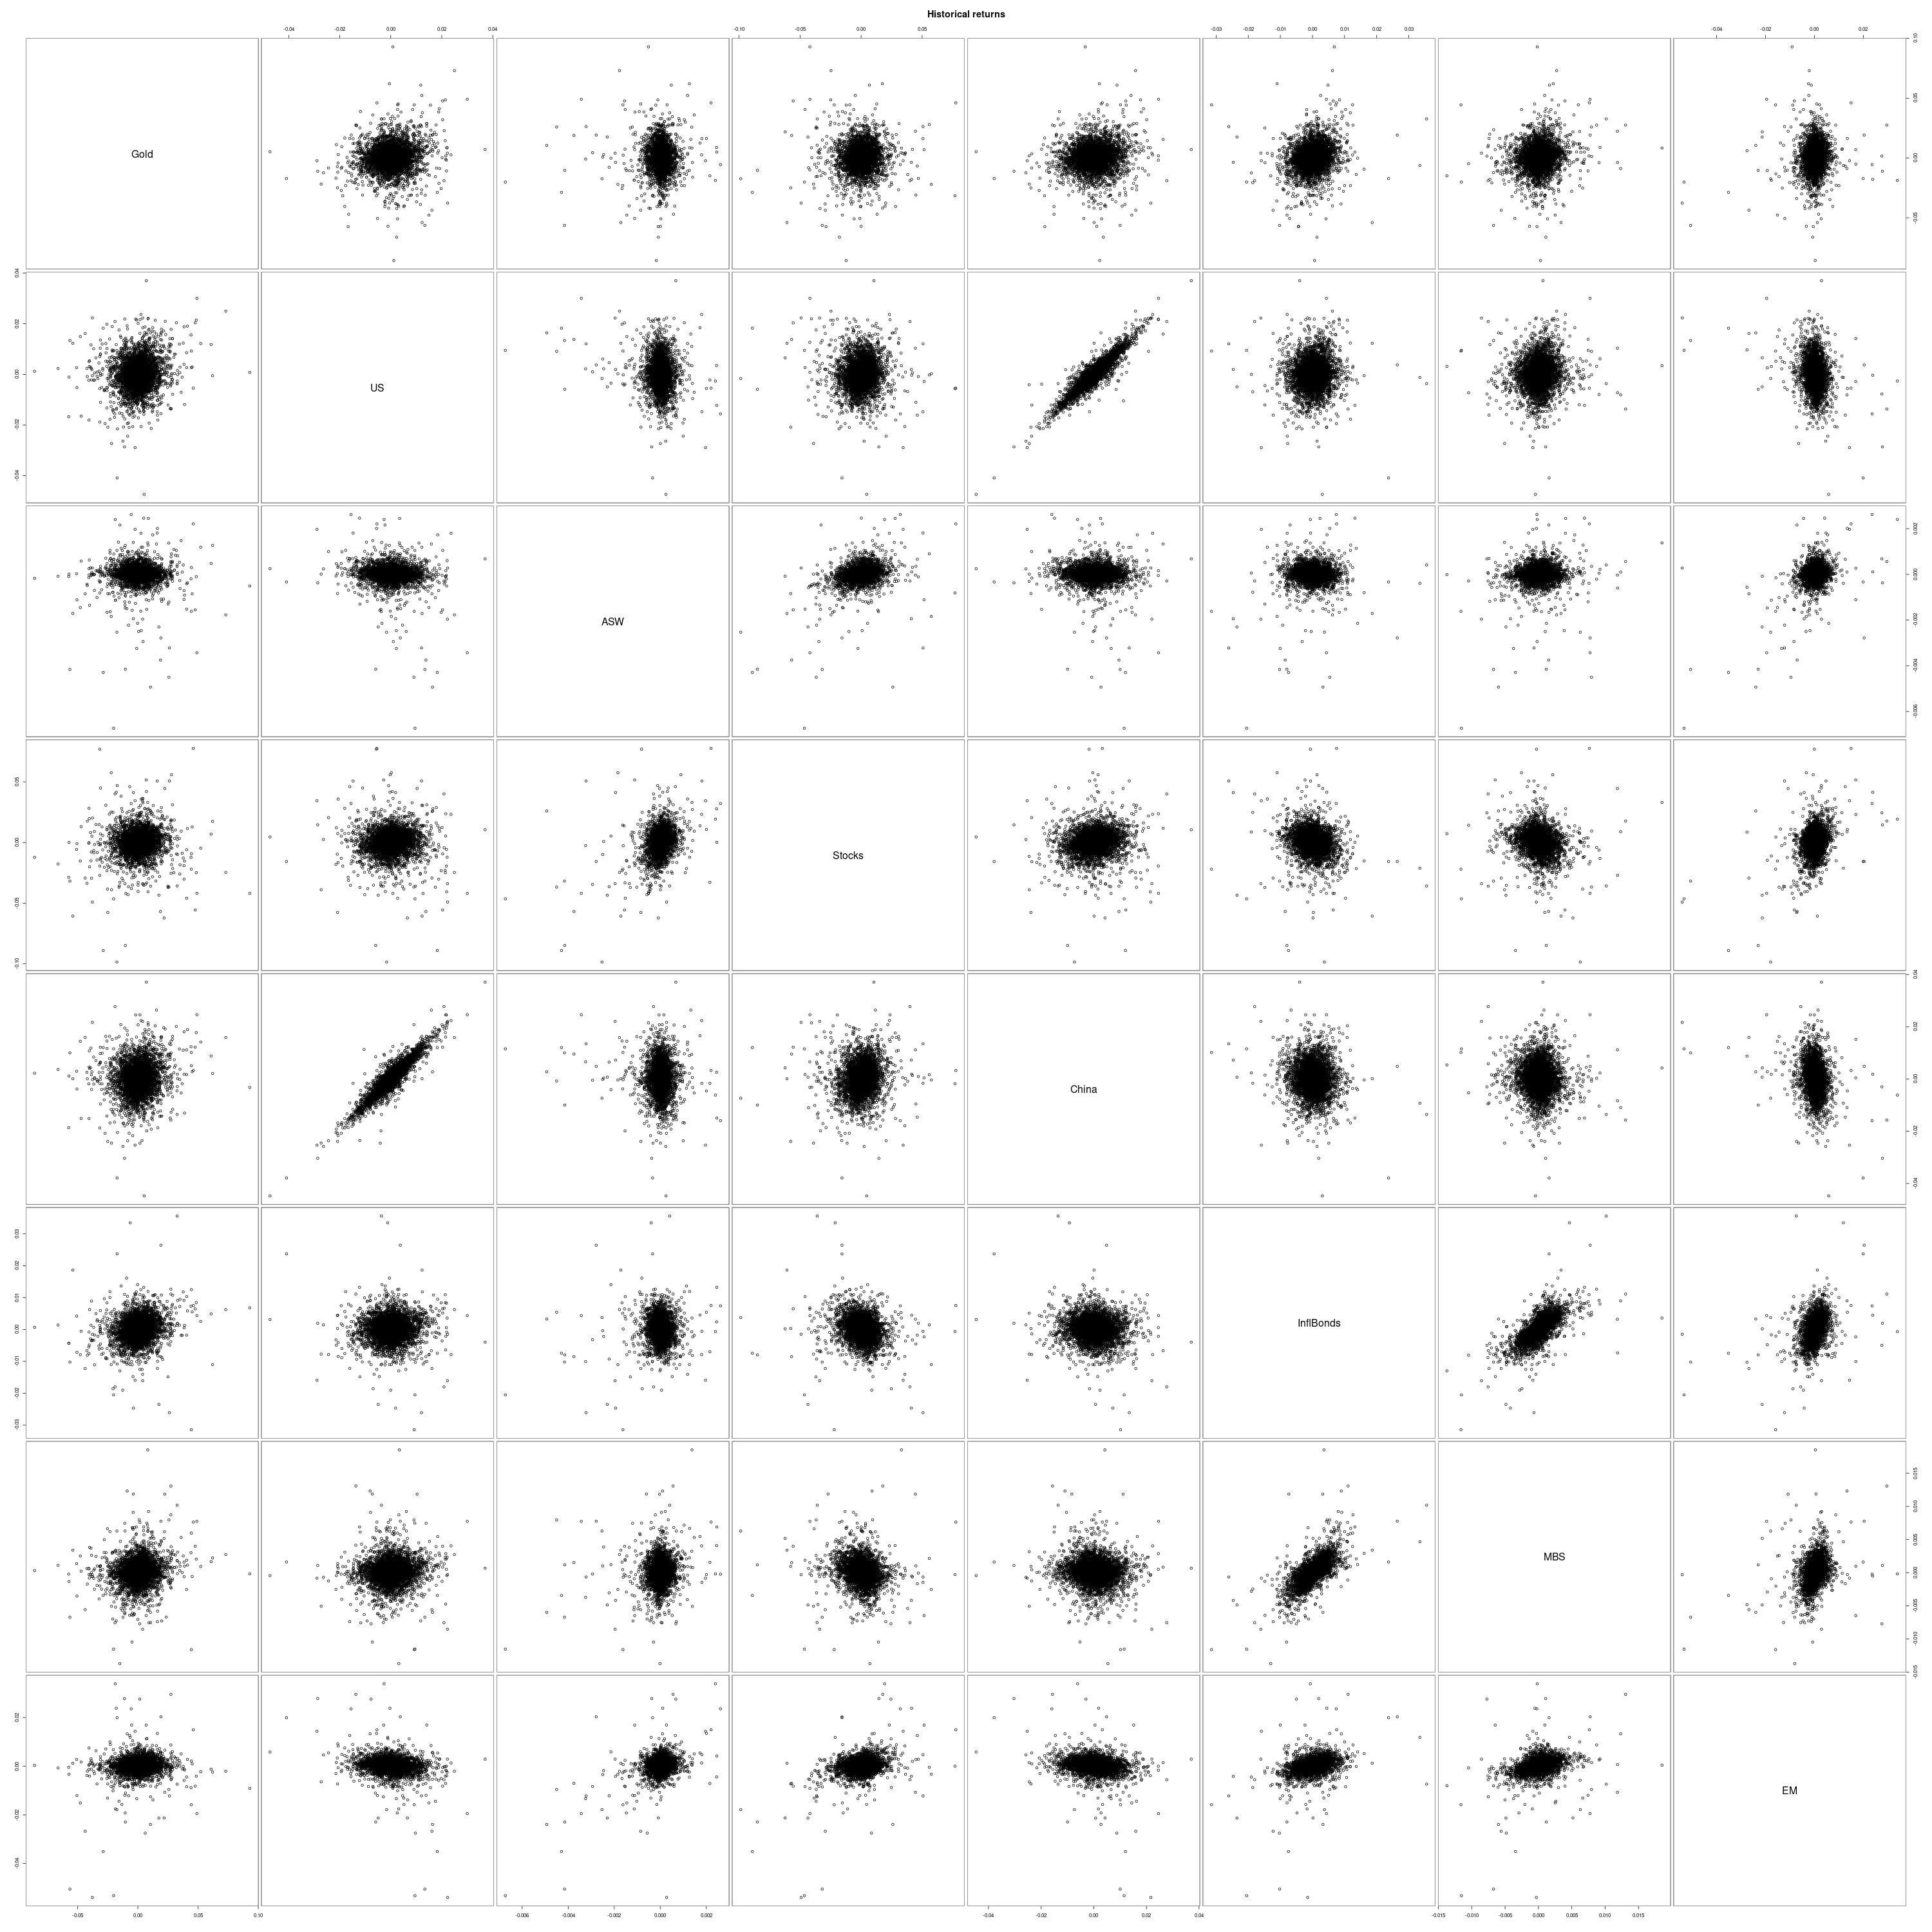
\includegraphics[width=\textwidth]{\detokenize{figures/correlations/Historical_Returns}}
		\caption{Historical returns}
	\end{subfigure}\\
	\begin{subfigure}{.75\columnwidth}
		\centering
		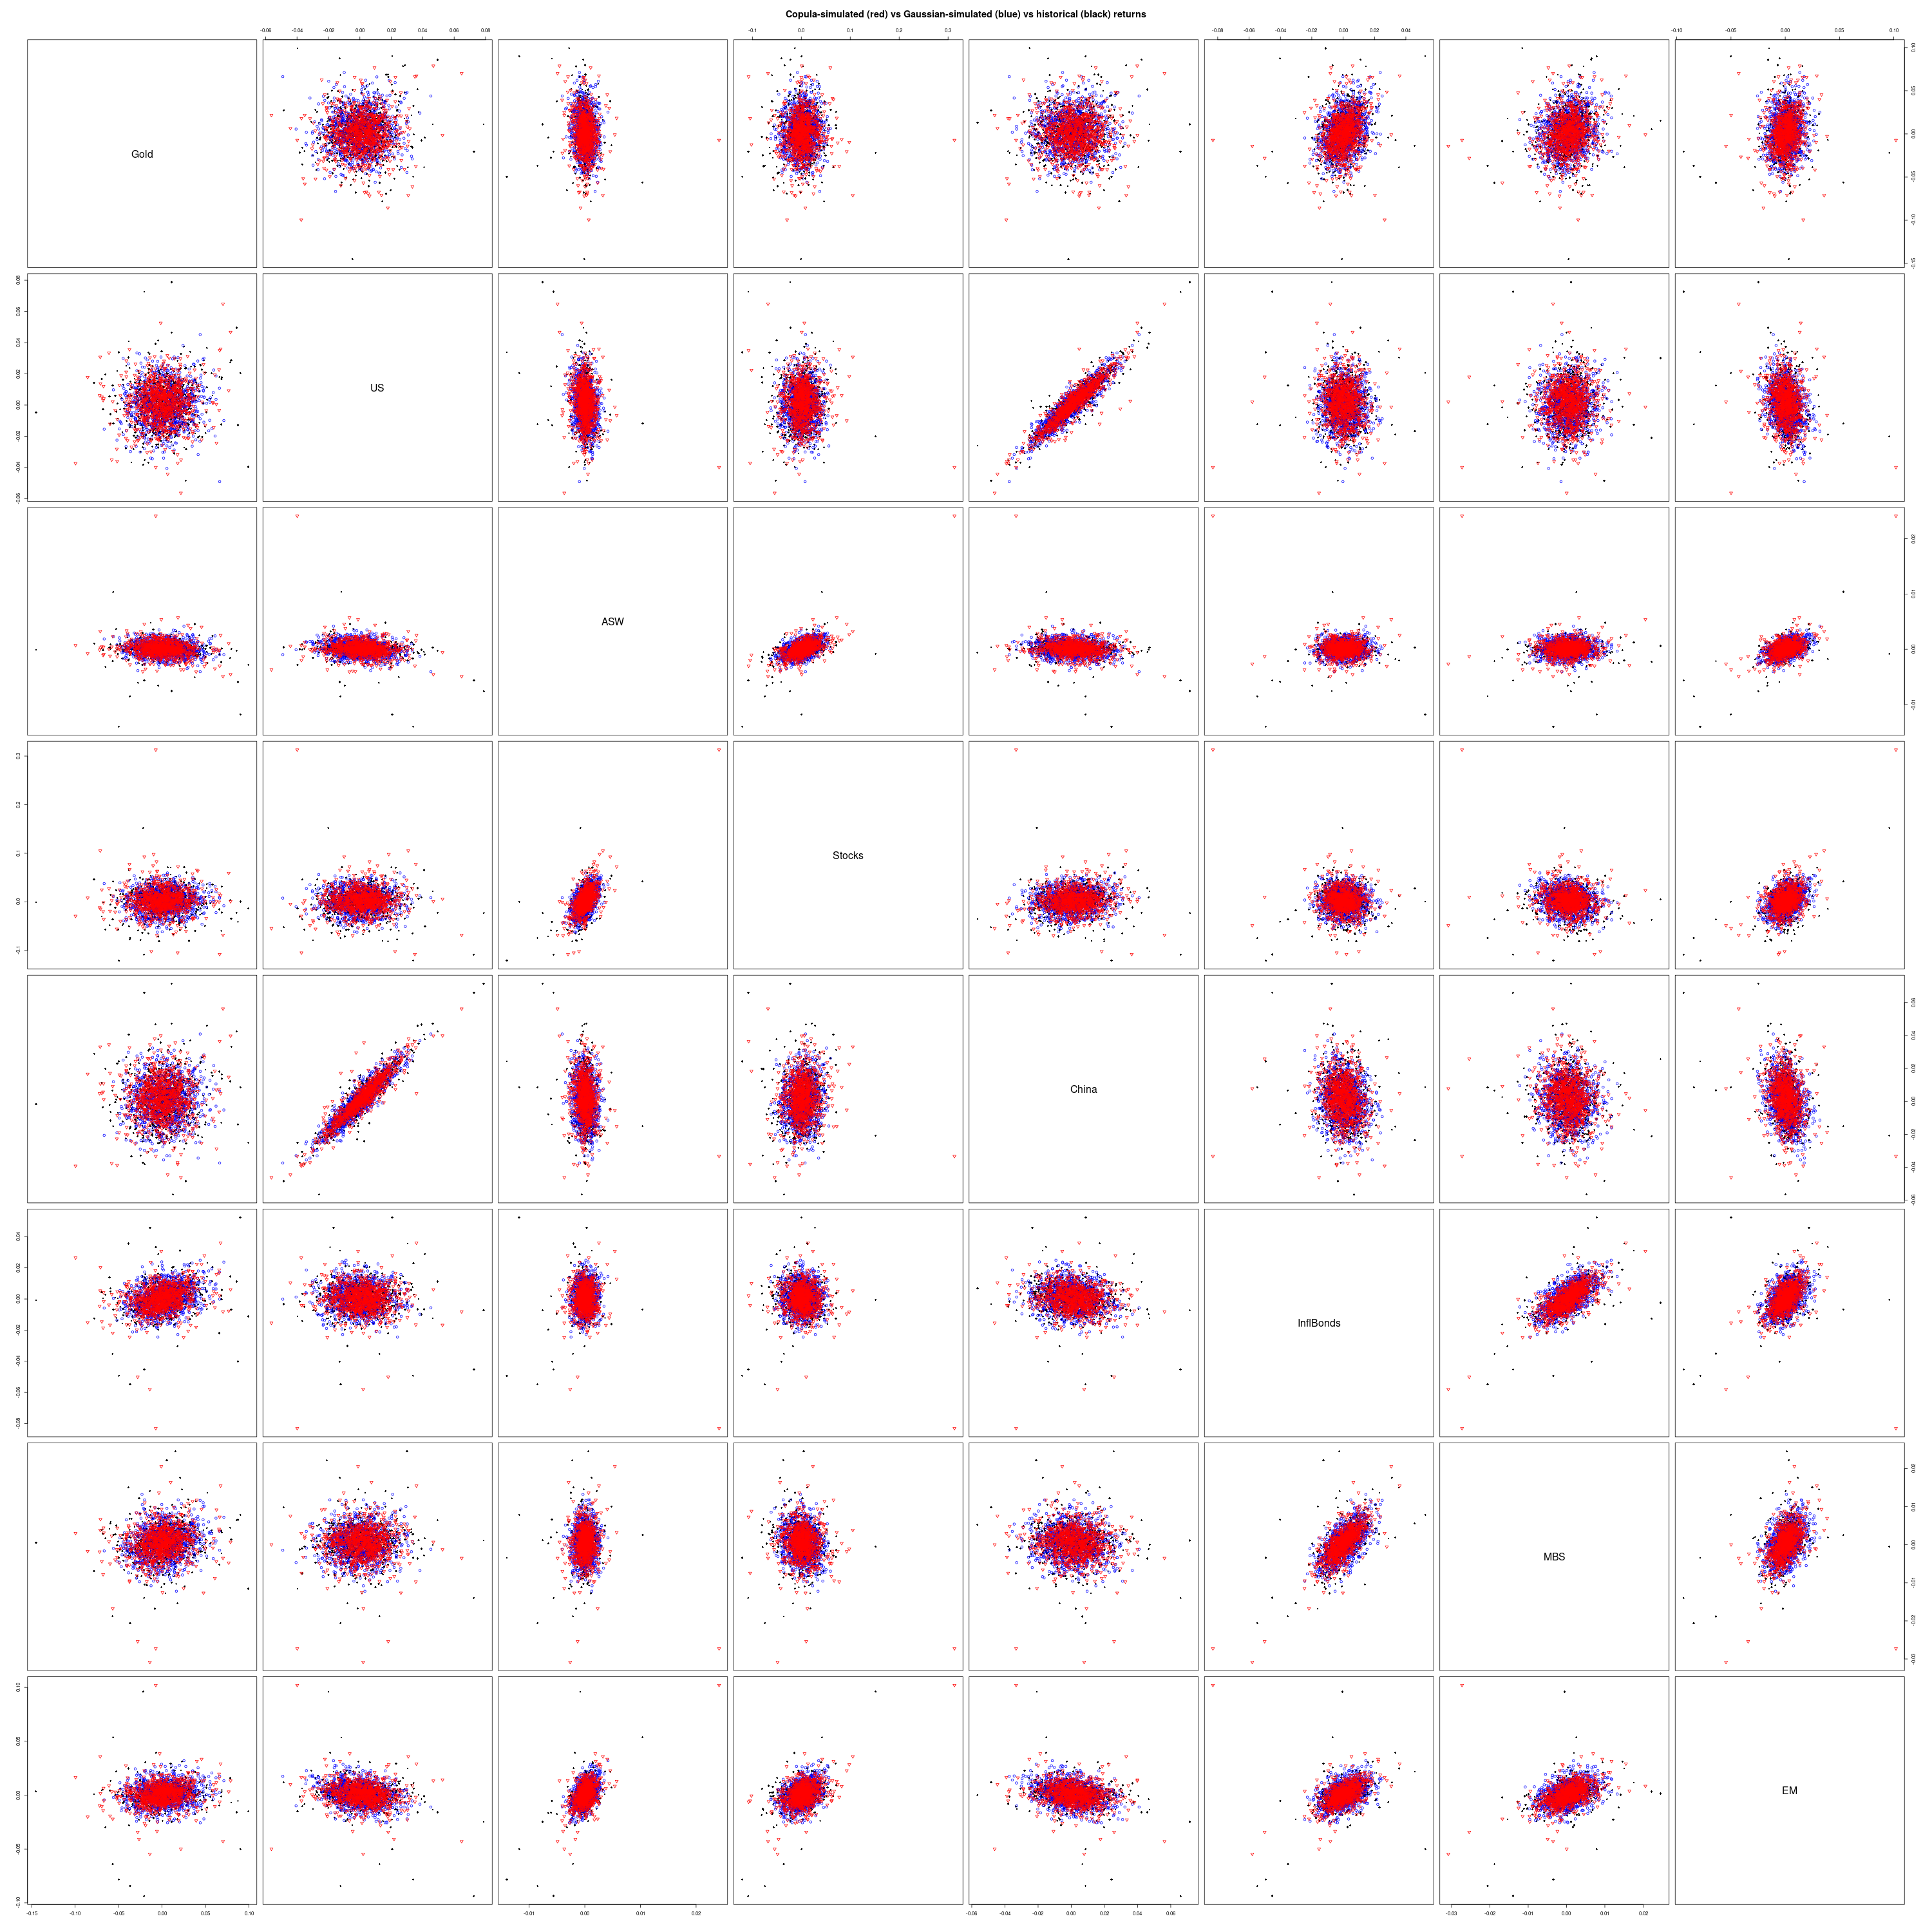
\includegraphics[width=\textwidth]{\detokenize{figures/correlations/Historical_vs_Gaussian_and_Pearson_returns3000}}
		\caption{Historical returns (black), Gaussian-distributed returns (blue) and Pearson-distributed returns(red)}
	\end{subfigure}
	\caption{Historical returns, density approximated with a Gaussian and Pearson distributions. Part 2/2}
	\label{fig:return_estimation:correlations}
\end{figure}

What we can see from the figures directly is that the Pearson-simulated returns are more clustered than the Gaussian-simulated returns, while exhibiting more outliers at the same time. This is due to the Pearson distribution, not the copula structure per se as the Pearson distribution allows us fatter tails than the Gaussian distribution.

In the next step, we examine the similarity between historical and simulated datasets by means of two different statistical tests - the Cramer test an the Kolmogorov-Smirnov test.

The Cramer test is a multi-dimensional test of distributional equality. It compares two distributions of multiple dimensions with each other and produces a test statistic and p-value corresponding to a null hypothesis $H0$ of equal distributions.

The Kolmogorov-Smirnov test on the other hand only looks at distributions of dimension one. Nevertheless, we can use it on our marginal distributions, so for each asset class separately.
Just like in the case of the Cramer test, the null hypothesis $H0$ in the Kolmogorov-Smirnov test also corresponds to the two distributions being equal.

In both tests, we will compare the simulated data with the historical data. We will do this separately for the Gaussian-simulated returns and for the Pearson-simulated returns. Results for both tests can be found in Table \ref{tab:return_estimation:KS_Cramer_testing}.

\begin{table}[h]
	\centering
	\begin{tabularx}{0.9\linewidth}{lXX}
		Test & Pearson distribution p-value & Gaussian distribution p-value\\
		\toprule
		Cramer test & 0.51 & 0.01 \\
		\toprule
		K-S test: Gold & 0.50 & 0.01 \\
		K-S test: US & 0.00 & 0.00 \\
		K-S test: ASW & 0.00 & 0.00 \\
		K-S test: Stocks & 0.99 & 0.12 \\
		K-S test: China & 0.41 & 0.00 \\
		K-S test: InfBonds & 0.06 & 0.00 \\
		K-S test: MBS & 0.00 & 0.00 \\
		K-S test: EM & 0.79 & 0.01 \\
		\bottomrule& 
	\end{tabularx}
	\caption{Testing of distributional equality on historical vs. Gaussian and historical vs. Pearson weekly returns.}
	\label{tab:return_estimation:KS_Cramer_testing}
\end{table} 

The Cramer test for distributional equality between historical and Pearson-simulated returns does not reject the null hypothesis of equal distributions. In the case of Gaussian distribution, the null hypothesis is rejected in favor of the alternative hypothesis $H1$, therefore showing that generating returns that are Pearson type VII distributed provides more superior results than a simple Gaussian approximation.

In the case of Kolmogorov-Smirnov test of marginal distributions, the results confirm the null hypothesis in 5 out of 8 asset classes for the Pearson-generated returns and only 1 out of 8 asset classes in the Gaussian-generated returns.

Both tests therefore suggest that using a Pearson type VII distribution allows us to better replicate historical returns than a simple Gaussian approximation.

The last step in this part of our algorithm is transforming the returns into the desired set of maturities and sample sizes and storing them in the dedicated folder structure. In this step, we also compute the relevant p.a. returns and store them as well.





